\section{Integration}
Disperate hardware timing channel protection mechanisms are not enough to 
implement a full, timing channel secure system. It requires support from 
software to manage the interaction of software entities with the hardware.  
Further, these hardware mechanisms are often interdependent. The shared cache 
miss path involves the cache, bus, and memory controller, all of which require 
timing channel protection. Haphazardly time multiplexing these resources can 
lead to unnecessarily large performance penalties or even total starvation. The 
integrated system requires carefully coordinating the protected resources. The 
rest of this section elaborates on the timing compartment manager, the software 
entitiy that initializes and manages timing compartments, and then describes 
how timing channel protection mechanisms should be coordinated.

\subsection{The Timing Compartment Manager}
\label{sec:integration_tcm}
The timing compartment manager (TCM) is responsible for initializing and 
managing timing compartments. At system initialization time it informs the 
hardware of the timing compartments present in the system and configures the 
hardware components with the policy. At run time, the TCM tags requests for 
shared hardware resources with the timing compartment ID (TCID) of the TC that 
originated the request. Shared hardware resouces then enforce the policy by 
checking the TCID before handling the request. The hardware allows software 
entities within the same compartment to share resources normally, and timing 
compartments can even be allocated multiple cores.

As shown in Figure \ref{fig:arch}, the timing compartments architecture is 
comprised of a set of $n$ cores which share resources. There is no limitation 
on $m$, the number of timing compartments that can reside in the system at one 
time. However, at most $n$ timing compartments can be active (executing on one 
or more physical cores) at a time. If $m>n$, active timing compartments must 
occasionally be switched with inactive ones. The TCM addresses this by context 
switching TCs according toa context switch schedule.

The TCM is implemented as an extension of the trusted software layer, such as 
the OS or hypervisor. It requires functions to handle the initialization
and context switching. It also requires a small address space of its 
own to store the register contents of inactive TCs and a queue of inactive TCs.
The rest of this section describes the hardware TCID storage elemnts controlled 
by the TCM, and then elaborates on how the TCM initializes the system and 
handles context switching.

\subsubsection{TCIDs}
\begin{figure}
    \begin{center}
        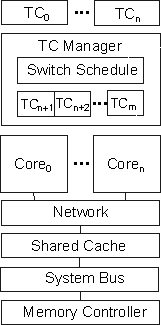
\includegraphics[width=1.08in]{figs/hw_sw_arch.pdf}
        \caption{The Timing Compartments Architecture}
        \label{fig:arch}
    \end{center}
\end{figure}

The hardware protection mechanisms track which timing compartment originated 
each request and handle the requests accordingly. To do so, requests (such as 
network packets or shared cache accesses) are tagged with a timing compartment 
ID (TCID). The set partitioned cache has $n$ registers which store the TCIDs
that own each of the (at most) $n$ partitions. When a request requires a 
replacement, the cache uses the TCID of the request to decide which partitions 
can allow entries to be replaced according to the policy. (Checking is only 
required on replacements since TCIDs have separate address spaces.) Each of the 
separate MSHR banks are tagged with a TCID of the owner, and requests can only 
affect the MSHR banks with the same TCID as the request. Each of the time 
multiplexed resources (the networks, the memory controller, shared cache 
response ports, and memory controller response ports) have $n$ queues. Each of 
these queues has a register to store the TCID which owns that particular queue, 
and time quanta are assigned to each queue. Lastly, each core has a register 
that stores the TCID of the TC currently active on that core. This is used to 
derive the tags that are appended to requests originating from that core. Table 
\ref{table:tcid} summarizes the TCID storage elements in the system.

\begin{table}
\begin{tabular}{l|l}
    \hline
    Component & TCID Storage \\
    \hline
    Core & $n$ cores. TCID register per core. \\
    Shared Cache Port & $n$ queues. TCID register per queue \\
    Shared Cache Parttitions & $n$ partition owner registers. \\
    Shared Cache MSHRs & $n$ MSHR banks. TCID per bank \\
    Network & $n$ queues. TCID register per queue\\
    \hline
\end{tabular}
    \caption{TCID storage for TC Architecture Components}
    \label{table:tcid}
\end{table}

\subsubsection{Initialization \& Handling Context Switches}
The TCM, initializes the system by setting the TCID storage elements listed in 
Table 1 with the IDs of the initially active timing compartments. At most $n$ 
of these can be active initially, so if $m>n$, some will be inactive, and the 
TCM must define a static context switching schedule at initialization time.

The time between context switches cannot depend on the dynamic behaviour of the 
TCs. Otherwise, a timing compartment could observe the time that they are 
context switched in or out to learn information about the timing compartment it 
is switched with. Instead, context switches occur at a fixed time interval, 
$T_{CTX}$. Every $T_{CTX}$ cycles the TCM is invoked to replace the timing 
compartment which has been active the longest with the TC at the head of the 
inactive TC queue. The compartment which has been switched out is moved to the 
back of the inactive TC queue.

To perform the context switch, the CPU pipeline and the memory request queue 
are drained. The general purpose registers of the outgoing TC are stored in 
TCM-space memory and tagged with the TCID. The private cache, shared cache 
partition, TLB, and branch predictor state of the outgoing TC are all flushed.  
Finally, the TCID stores of the outgoing TC are replaced with the TCID of the 
incoming TC. 

The time required to perform a context switch depends on the state and behavior 
of the outgoing TC. The owner of the incoming TC can observe when the incoming 
TC begins executing, so this implies a potential leakage of secrets.  To 
prevent this, context switches are bound to always take the worst case time.  
If a context switch completes early, the incoming TC is stalled until the worst 
case context switch time has been reached.

\subsection{Coordination}
